\documentclass[12pt]{article}
\usepackage[margin=0.8in]{geometry}
\usepackage{amsmath}
\usepackage{hyperref}
\usepackage{graphicx}
\usepackage{float}
\usepackage{caption}
\usepackage{subcaption}

\title{Numerical analysis: Assignment 5}
\author{Niccolo Zuppichini}
\begin{document}

\maketitle
\section*{Exercise 1}

Given a Bernstein polynomial $B^n_i =  \binom{n}{i} (1-s)^{n-i} s^i$, then it's derivative is given by: \\


$$(B^n_i)'(s) = D(\binom{n}{i} (1-s)^{n-i} s^i) = $$

Because $\binom{n}{i} $ is a constant we can take it out: \\

$$ = \binom{n}{i}  D \bigg( (1-s)^{n-i} s^i) \bigg) = $$

By taking the derivative using the chain rule, it follows: \\

$$ =  \binom{n}{i}  \bigg( i s^{i-1} (1-s)^{n-i} + s^i (n-i) (1-s)^{n-i-1} (-1) \bigg) = $$

By rearranging: \\

$$ = \binom{n}{i}  \bigg( i s^{i-1} (1-s)^{n-i} - s^i (n-i) (1-s)^{n-i-1}  \bigg) = $$

By definition of the newton binomial: \\

$$ = \frac{n!}{i! (n-i)!} \bigg( i s^{i-1} (1-s)^{n-i} - s^i (n-i) (1-s)^{n-i-1}  \bigg) = $$ 

It follows: \\

$$ =  \bigg(\frac{n!}{i! (n-i)!} i s^{i-1} (1-s)^{n-i} - \frac{n!}{i! (n-i)!} s^i (n-i) (1-s)^{n-i-1}  \bigg) = $$

$$ =  \bigg(\frac{n!}{(i-1)! (n-i)!} s^{i-1} (1-s)^{n-i} - \frac{n!}{i! (n-i-1)!} s^i (1-s)^{n-i-1}  \bigg) =$$

$$ = \bigg(n \frac{(n-1)!}{(i-1)! (n-i)!}  s^{i-1} (1-s)^{n-i} - n \frac{(n-1)!}{i! (n-i-1)!} s^i (1-s)^{n-i-1}  \bigg) =$$

$$ = n \bigg(\frac{(n-1)!}{(i-1)! (n-i)!} (1-s)^{n-i} s^{i-1} - \frac{(n-1)!}{i! (n-i-1)!}   (1-s)^{n-i-1} s^i \bigg) =$$

Observe that the two factors inside the big brackets are given by $B_{i-1}^{n-1}$ and $B_{i}^{n-1}$, therefore: \\

$$ n \bigg(B_{i-1}^{n-1}(s) - B_{i}^{n-1}(s)  \bigg) = (B^n_i)'(s)$$

Concluding the proof. \\

\section*{Exercise 2}

\begin{figure}[H]
	\centering
	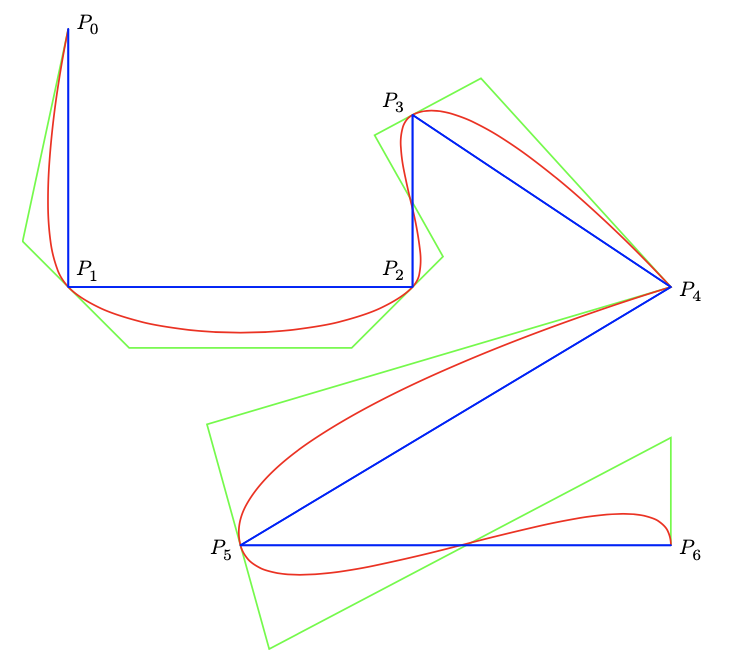
\includegraphics[width=0.7\columnwidth]{exercise2.png}
	\caption{The piecewise spline}
	\label{fig:ex2}
\end{figure}

In my opinion, this is a combination of two splines, joining in the point $P_4$: one going through the points $P_0, P_1, P_2, P_3, P_,4$ and a second one through $P_4, P_5, P_6$. The two splines are composed of many cubic bezier curves satisfying the following conditions for each pair of points $P_i, P_{i+1}$:

\begin{enumerate}
	\item The transition around $P_i$ is smooth $\forall \; i \in [0, 6]$
	\item The curvature on the boundary points is zero
\end{enumerate}

The first condition is given by ensuring that $(B^n_{i}(t=0))' = (B^n_{i-1}(t=1))'$ and along with $(B^n_{i}(t=0))'' = (B^n_{i-1}(t=1))''$ it ensures smoothness around the points $P_i$. \\

The first derivative is given by (I took it from wikipedia \footnote{\url{https://en.wikipedia.org/wiki/Bezier_curve#Cubic_Bezier_curves}}): 

$$B_i' = 3(1-t)^{2} (P_1 - P_0) +6(1-t)t( P_{2}- P_{1})+3t^{2}(P_{3}- P_{2})$$  

where $P_1$ and $P_2$ are the unknowns (i.e. the green handlers) and $P_0$ and $P_3$ are given (blue points). Let's call $P_1$ and $P_2$ a, b for clarity. Then: \\

$$B_i' = 3(1-t)^{2} (a - P_i) +6(1-t)t(b - P_{i+1})+3t^{2}(P_{i+1} - b)$$  

By employing the first order condition: \\
\begin{equation}
	(B_{i-1}(t=1))' = (B_i(t=0))'
	\label{eq:first_condition}
\end{equation}
$$\implies a_i + b_{i-1} = 2 P_i$$
\\
The second derivative (took it from wikipedia as well) is given by: \\
$$B_i'' = 6(1-t) (b - 2 a + P_i) + 6t (P_{i+1} -2 b + a) $$
By employing the second order condition: \\

\begin{equation}
	(B_{i-1}(t=1))'' = (B_i(t=0))''
	\label{eq:eq:second_condition}
\end{equation}
%$$ P_{i} -2 b_{i-1} + a_{i-1}  = P_{i} -2 a_i + b_i) $$
$$ \implies  a_{i-1} + 2 a_i = 2 b_{i-1} + b_i $$
\\
% Explain why to add this condition
Then for the boundaries: \\
$$(B_0 (t=0)'' = 0$$
%$$\implies  b_0 - 2 a_0 + P_0 = 0 $$

$$\implies 2 a_0 -b_0 = P_0 $$

$$(B_{n-1} (t=1)'' = 0)$$
% P_{n} -2 b_{n-1} + a_{n-1} = 0
$$ \implies  a_{n-1} -2 b_{n-1} + P_{n} = 0 $$

We end up with a system of equations: \\
\begin{equation}
\begin{cases}
a_i + b_{i-1} = 2 P_i \\
a_{i-1} + 2 a_i = 2 b_{i-1} + b_i  \\
2 a_0 -b_0 = P_0  \\
a_{n-1} -2 b_{n-1} + P_{n} = 0
\end{cases}
\textrm{for} \; i \in [1, n-1]

\label{eq:system}	
\end{equation}

The goal now is to express the system as a matrix-vector product. Therefore we must explicit one of unknowns (a or b) in function of the other. I choose to express $b$ in function of $a$ because it looked easier to do (note how now the index i goes from 0 to n-2 rather than 1 to n-1):

$$b_i = 2 P_{i+1} - a_{i+1} \forall i \in [0, n-2]$$  \\
Then: \\
$$
\begin{cases}
b_i = 2 P_{i+1} - a_{i+1} \\
a_{i-1} + 2 a_i = 2 (2 P_i - a_i) + 2 P_{i+1} - a_{i+1}  \\
2 a_0 - (2 P_{1} - a_{1}) = P_0  \\
a_{n-1} -2 b_{n-1} + P_{n} = 0
\end{cases}
=
\begin{cases}
b_i = 2 P_{i+1} - a_{i+1} \\
a_{i-1} + 4 a_i + a_{i+1}= 4 P_i + 2 P_{i+1}  \\
2 a_0 + a_1 = P_0 + 2 P_1  \\
a_{n-1} -2 b_{n-1} + P_{n} = 0
\end{cases}
i \in [1, n-1]
$$

We can't insert $b_i$ into the fourth equation because it's not defined for $n-1$, but we can use the second equation from the system of equations\ref{eq:system} and re-arrange it for $b_{n-1}$: \\

$$
b_{n-1} = - 2 b_{n-2} + a_{n-2} + 2 a_{n-1}
$$
Then:

$$
a_{n-1} -2 (- 2 b_{n-2} + a_{n-2} + 2 a_{n-1}) + P_{n} = 4 b_{n-2} -2 a_{n-2} -3 a_{n-1} + P_{n} =
$$
$$ =4 (2 P_{n-1} - a_{n-1}) -2 a_{n-2} -3 a_{n-1} + P_{n} = 8 P_{n-1} - 7 a_{n-1} -2 a_{n-2} + P_n = 0$$

We can finally write the final system of equation:

\begin{equation}
\begin{cases}
b_i = 2 P_{i+1} - a_{i+1} \\
a_{i-1} + 4 a_i + a_{i+1}= 4 P_i + 2 P_{i+1}  \\
2 a_0 + a_1 = P_0 + 2 P_1  \\
7 a_{n-1} + 2 a_{n-2} = P_n + 8 P_{n-1}
\end{cases}
i \in [1, n-1]
\label{eq:final}
\end{equation}


Writing this system of equations as a linear system in the form $B a = P$ is now trivial. $B$ is a tridiagonal matrix that employs the relations \ref{eq:system} of the variable, $a$ is a vector containing all the unknowns (i.e. $a = [a_0 ... a_{n-1}]$ and $P$ another vector containing the data points. I have implemented the system in python and solved it, however, I did not get the same results as adobe illustrator. \\

\begin{figure}[H]
\centering
\begin{subfigure}{.5\textwidth}
  \centering
	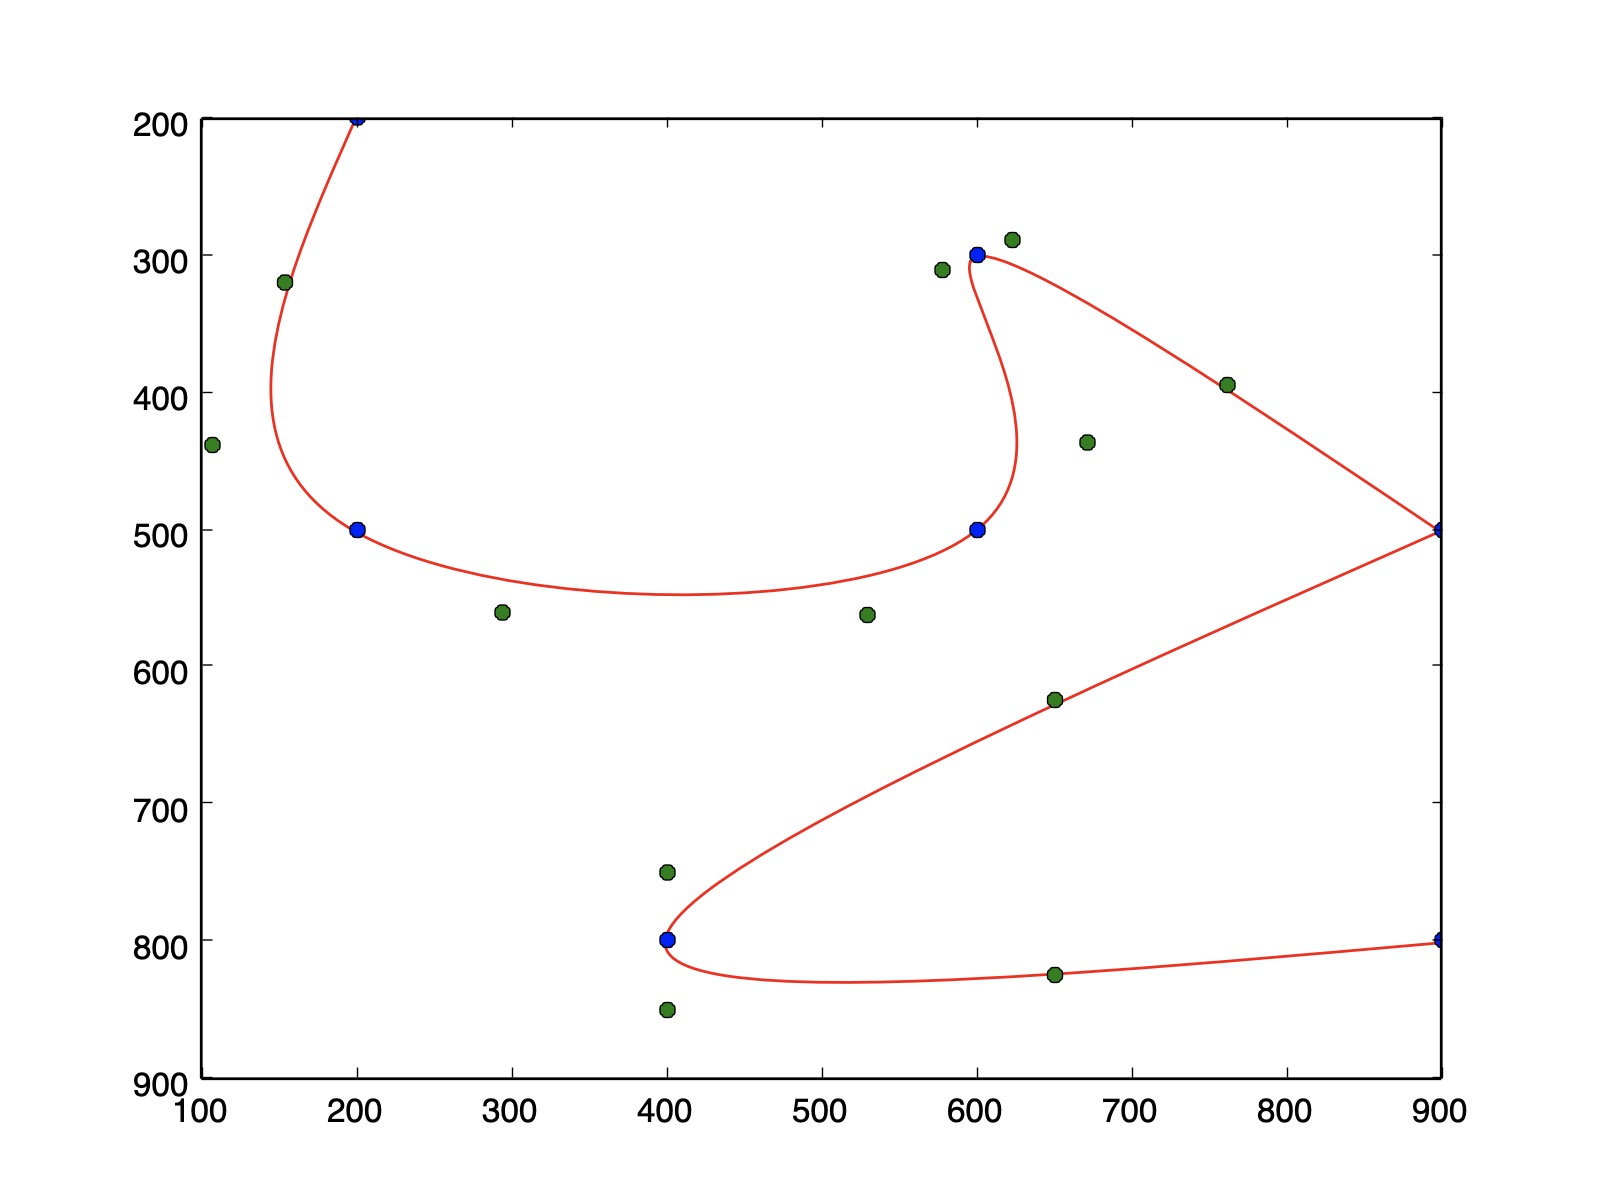
\includegraphics[width=0.7\columnwidth]{result.jpg}
	\caption{The red curve is my spline, the blue points the data points and the green points the handlers A, B I've computed}
	\label{fig:result}
\end{subfigure}%
\begin{subfigure}{.5\textwidth}
 \centering
	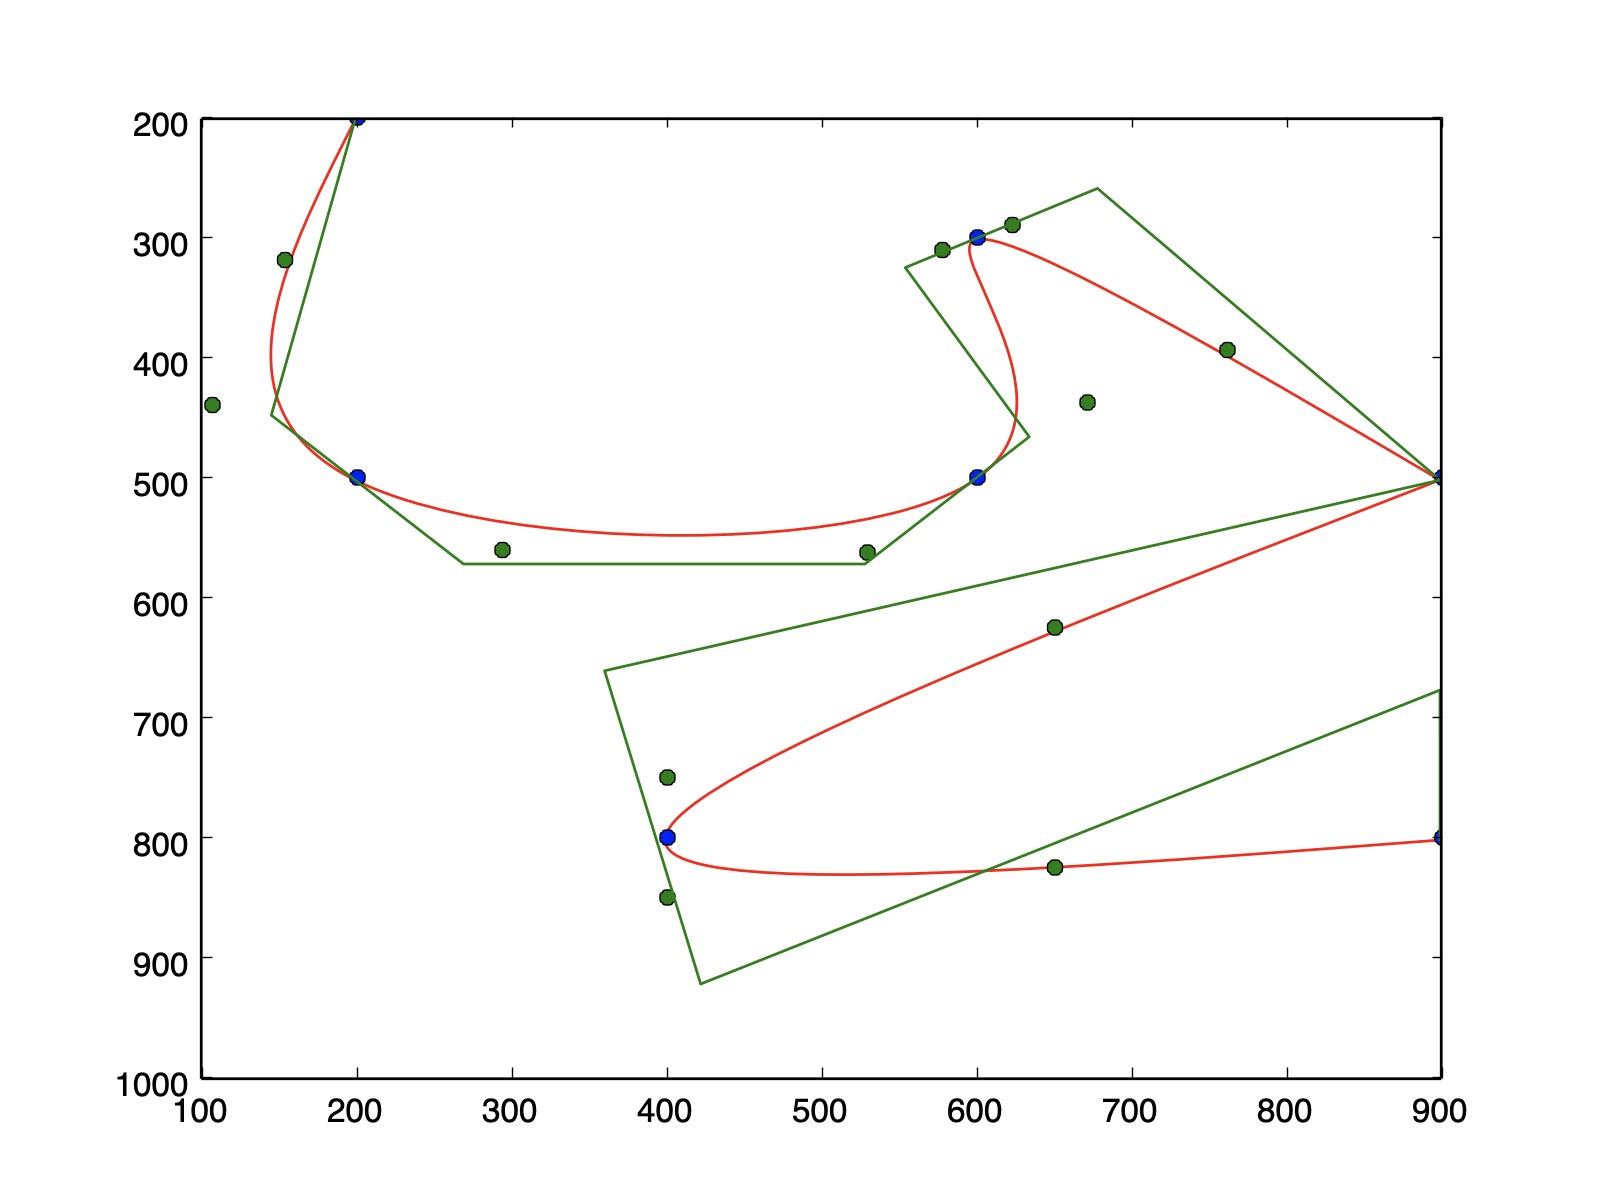
\includegraphics[width=0.7\columnwidth]{convex_hull.jpg}
	\caption{Same plot but shows also the same green convex hull given in the assignment}
	\label{fig:result}
\end{subfigure}
\caption{Result from my python implementation. }
\label{fig:test}
\end{figure}

Figure \ref{fig:result} clearly shows that my piecewise cubic bezier doesn't agree with the green convex hull (i.e. a bezier should always be inside its convex hull) therefore it's clear that my implementation differs from the one adobe illustrator uses, however, the idea behind it (i.e. satisfy first and second-order conditions) probably agrees with mine. In conclusion, I think that adobe illustrator implementation differs on the way they treat the boundary points (i.e. $P_0$, $P_4$ and $P_6$) but I'm unsure about how they do it. \\

The python code can be found in the folder \textit{code}. \\
%result
%https://towardsdatascience.com/b%C3%A9zier-interpolation-8033e9a262c2
%https://stackoverflow.com/questions/5634460/quadratic-b%C3%A9zier-curve-calculate-points


\end{document}